\documentclass[11pt,aspectratio=169]{beamer}
\usetheme{Madrid}
\usefonttheme{serif}
\setbeamercolor{background canvas}{bg=white}
\setbeamersize{text margin left=0.5cm, text margin right=0.5cm}

\usepackage{fontspec}
\usepackage{xeCJK}
\setCJKmainfont{Microsoft YaHei} % 使用微软雅黑作为中文主字体


\usepackage[scheme=plain]{ctex}
\usepackage{amsmath}
\usepackage{amsfonts}
\usepackage{amssymb}
\usepackage{graphicx}

\DeclareMathOperator{\sen}{sen}
\DeclareMathOperator{\tg}{tg}

\setbeamertemplate{caption}[numbered]

\author[陈振源]{陈振源 \\ 指导老师:刘仁义, 张丰}
\title{基于扩散模型的高效灾害遥感图像文本控制生成和应用}
% Informe o seu email de contato no comando a seguir
% Por exemplo, alcebiades.col@ufes.br
\newcommand{\email}{bili\_sakura@zju.edu.cn}
%\setbeamercovered{transparent} 
\setbeamertemplate{navigation symbols}{} 
% \logo{
\includegraphics[scale=0.08]{imagens/logomarca_profmat.png}} 
\institute[]{浙江大学地球科学学院} 
\date{\today} 
%\subject{}

% ---------------------------------------------------------
% Selecione um estilo de referência
\bibliographystyle{apalike}

%\bibliographystyle{abbrv}
%\setbeamertemplate{bibliography item}{\insertbiblabel}
% ---------------------------------------------------------

% ---------------------------------------------------------
% Incluir os slides nos quais as referências foram citadas
%\usepackage[brazilian,hyperpageref]{backref}

%\renewcommand{\backrefpagesname}{Citado na(s) página(s):~}
%\renewcommand{\backref}{}
%\renewcommand*{\backrefalt}[4]{
%	\ifcase #1 %
%		Nenhuma citação no texto.%
%	\or
%		Citado na página #2.%
%	\else
%		Citado #1 vezes nas páginas #2.%
%	\fi}%
% ---------------------------------------------------------

\begin{document}

\begin{frame}
\titlepage
\end{frame}

\begin{frame}{大纲}
\tableofcontents 
\end{frame}

\section{背景介绍和研究目标}
\begin{frame}{背景介绍与研究目标}
\begin{block}{背景介绍}
    \begin{itemize}
        \item 自然灾害不可预测,遥感影像对救灾关键
        \item 现有高分辨率双时相灾害遥感图像稀缺
        \item 传统与文本引导方法难以生成真实、语义一致的遥感影像
    \end{itemize}
\end{block}
\begin{block}{研究目标}
    \begin{itemize}
        \item 利用扩散模型进行图像生成(编辑)
        \item 使用灾前图像和文本描述进行可控生成
    \end{itemize}
    \begin{center}
        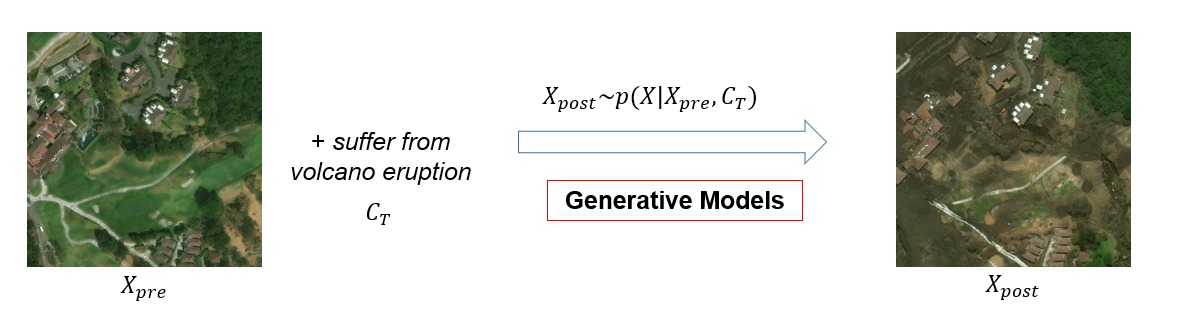
\includegraphics[width=0.5\linewidth]{imagens/diffusion_editing.png}\\
        \small 研究目标示意图
    \end{center}
\end{block}
\end{frame}

\section{数据集和模型方法}
\begin{frame}{数据集}
    \begin{columns}
        \begin{column}{0.6\textwidth}
            \begin{figure}
                \centering
                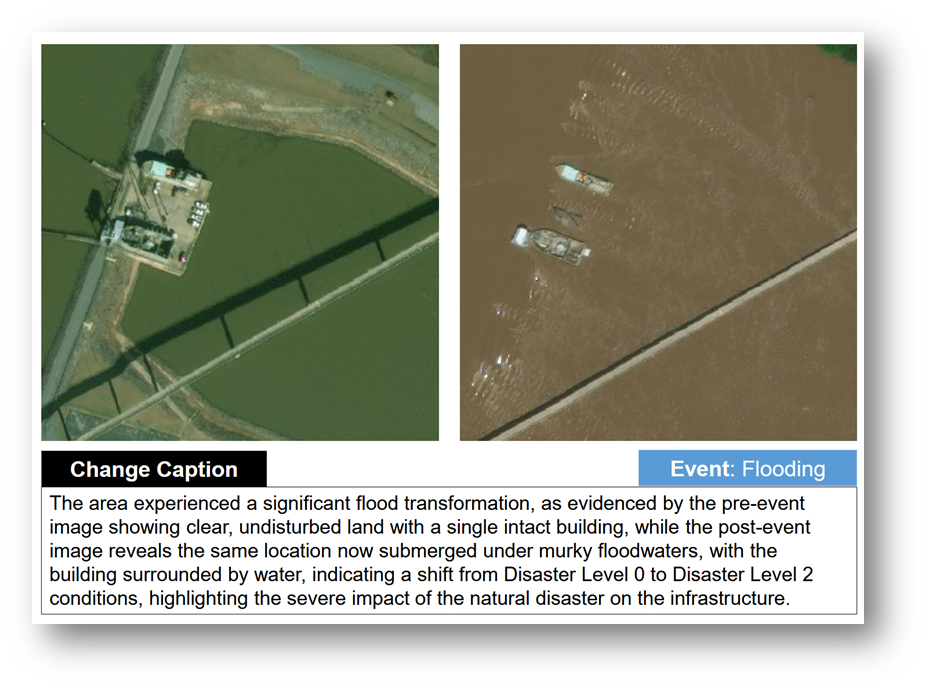
\includegraphics[width=0.9\linewidth]{imagens/rscc.png}

                {\tiny \textbf{RSCC数据集~\cite{chenRSCC2025}。该数据集包含62,351对事件前后遥感图像(512×512像素)及详细的变化描述文本。包含31次不同灾害事件。}}
            \end{figure}
        \end{column}
        \begin{column}{0.5\textwidth}
            \begin{figure}
                \centering
                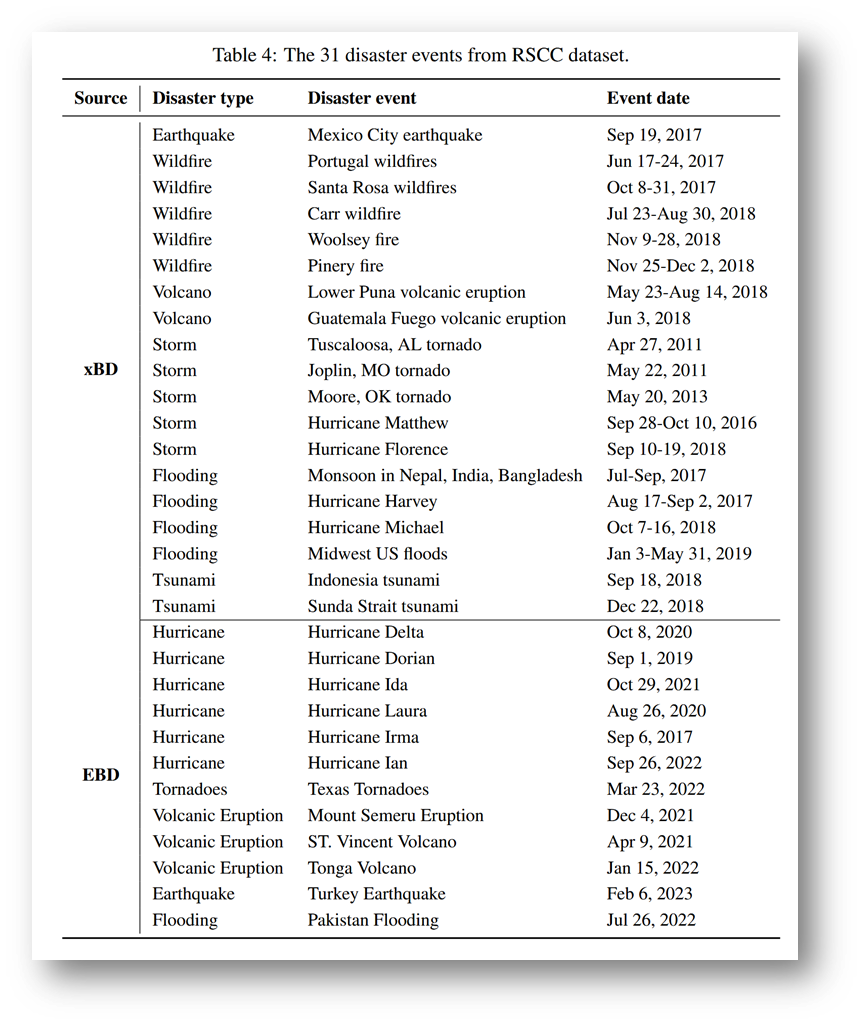
\includegraphics[width=0.8\linewidth]{imagens/rscc2.png}
            \end{figure}
        \end{column}
    \end{columns}
    \begin{flushleft}
        {\tiny \textcolor{gray}{\textit{Chen et al., RSCC: A Large-Scale Remote Sensing Change Caption Dataset for Disaster Events, submit to NeurIPS 2025 Dataset and Benchmark track (under review), 2025
        }}}
    \end{flushleft}
\end{frame}

\begin{frame}{基线模型框架}
    \begin{columns}
        \begin{column}{0.4\textwidth}
            {\tiny
            \begin{itemize}
                \item InstructPix2Pix~\cite{Brooks_2023_CVPR}
                \item UltraEdit~\cite{zhaoUltraEditInstructionbasedFineGrained2024b}
                \item Step1X-Edit~\cite{liuStep1XEditPracticalFramework2025}
                \item ICEdit~\cite{zhangInContextEditEnabling2025}
                \item ICEdit框架:通过上下文提示词实现零样本指令遵循,无需结构性修改。LoRA-MoE混合微调策略:高效适应与动态专家路由,提升灵活性,无需大规模再训练。推理时早期筛选方法:利用视觉-语言模型(VLM)在早期选择更优初始噪声,提升编辑质量。
            \end{itemize}
            }
        \end{column}
        \begin{column}{0.6\textwidth}
            \centering
            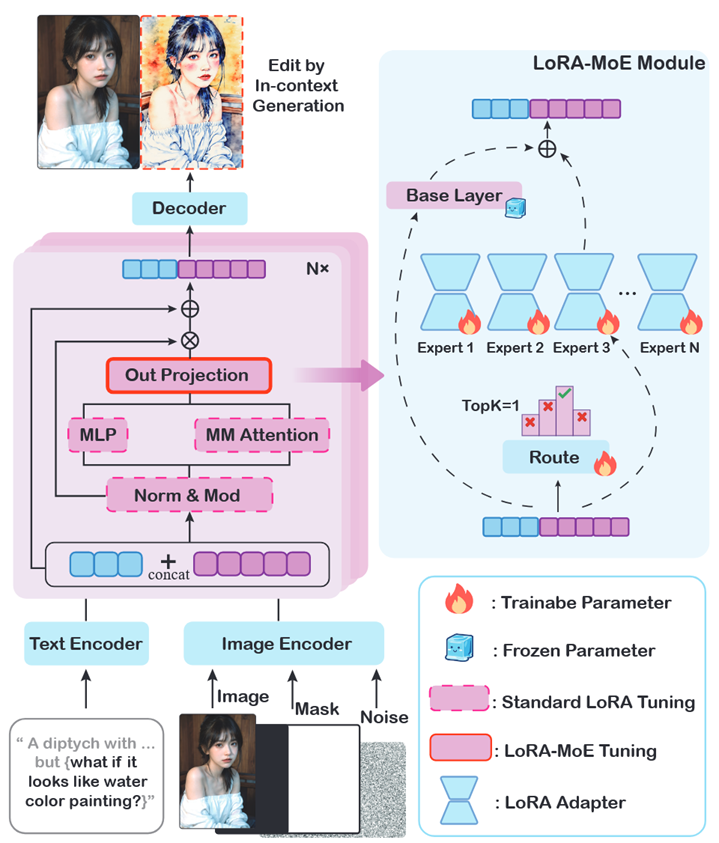
\includegraphics[width=0.65\linewidth]{imagens/icedit_framework.png}

            {\tiny \textbf{现有图像编辑框架ICEdit架构示意图~\cite{zhangInContextEditEnabling2025}}}
        \end{column}
    \end{columns}
\end{frame}

\begin{frame}{初步实验结果(基线模型)}
    \centering
    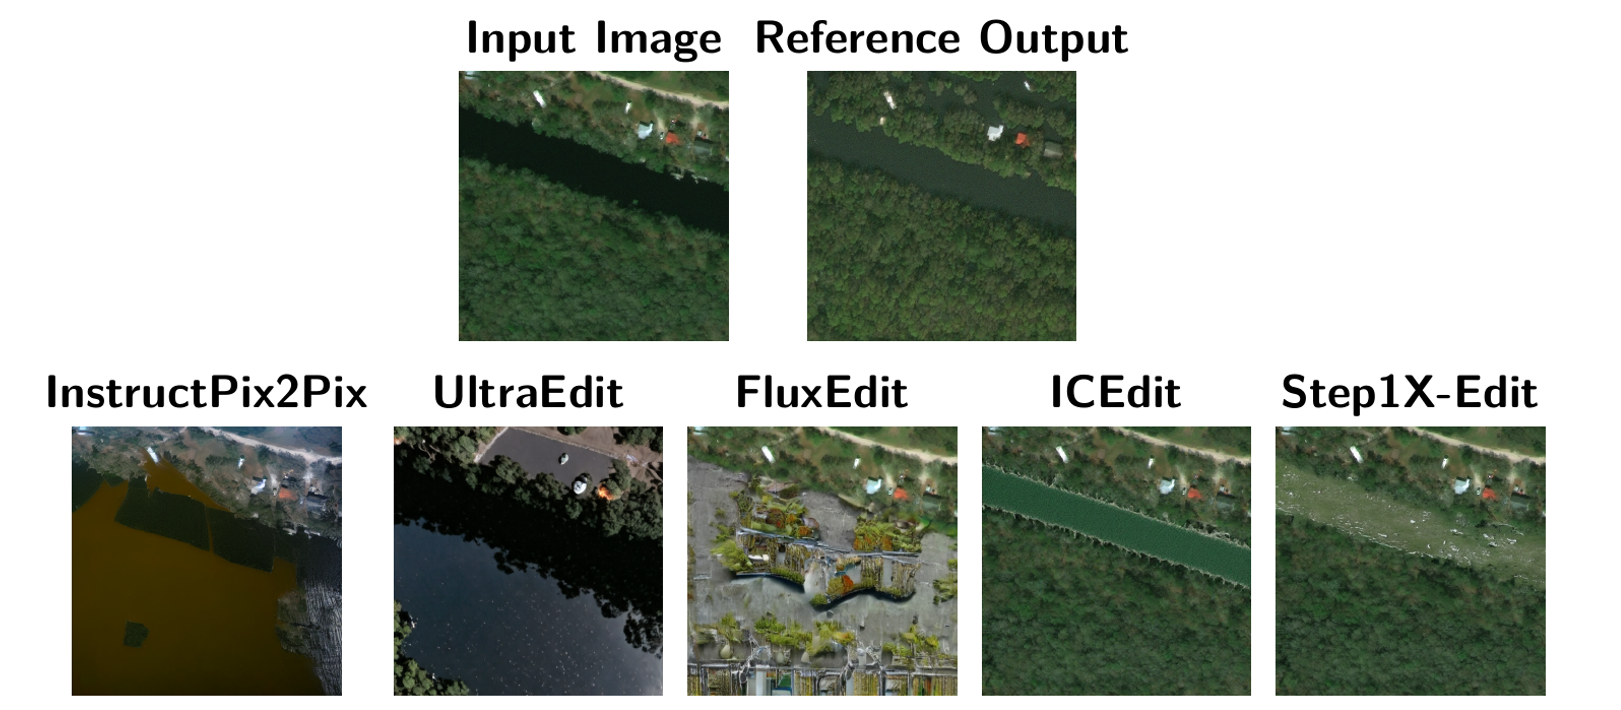
\includegraphics[width=0.95\linewidth]{imagens/baseline_results.png}
    % \vspace{0.2cm}
    
    {\tiny
    不同图像编辑模型(未经微调)的结果。\\
    \textbf{提示词:}“在最近的卫星图像对比中,观测到显著变化:水位明显上升,淹没了之前可见的部分陆地,极大地改变了景观外观。”
    }
\end{frame}

\begin{frame}{下游任务应用:数据增广方法对比}

    \textbf{传统数据增强方法}
    \begin{itemize}
        \item \textbf{主要技术}
        \begin{itemize}
            \item 几何变换,颜色扰动,噪声注入
            \item Cutout~\cite{devriesImprovedRegularizationConvolutional2017}
            \item CutMix~\cite{yunCutMixRegularizationStrategy2019}
            \item Copy-Paste~\cite{ghiasiSimpleCopyPasteStrong2021}
        \end{itemize}
        \item \textbf{相关研究~\cite{steinerHowTrainYour2022}讨论了各种数据增广方式对ViT分类精度提升效果。}
    \end{itemize}
    \vspace{0.3em}
    
    \textbf{合成数据增广在图像分类中的应用} \\
    前人研究发现~\cite{heSyntheticDataGenerative2022}通过生成合成遥感图像及其变化描述,可用于扩充有限的真实数据集,提升下游图像分类模型的泛化能力。
\end{frame}

\section{当前进展}
\begin{frame}{当前进展}
    \begin{columns}
        \begin{column}{0.48\textwidth}
            \textbf{当前完成项~\checkmark}
            \begin{itemize}
                \item 数据集准备完成
                \item 基线模型训练代码开发
                \item 基线模型推理代码开发
                \item 单模型最小化训练测试验证
            \end{itemize}
        \end{column}
        \begin{column}{0.04\textwidth}
        \end{column}
        \begin{column}{0.48\textwidth}
            \textbf{进行中任务}
            \begin{itemize}
                \item 评估指标开发(部分完成)
                \item 大规模消融实验设计
                \item 下游任务应用(基于数据增强的图像分类)
            \end{itemize}
        \end{column}
    \end{columns}
\end{frame}


% \section{Reference}
\begin{frame}[allowframebreaks]{参考文献}
    \bibliography{referencias}
\end{frame}


\end{document}